\resizebox{10cm}{!}{%
\usetikzlibrary{shapes.geometric}
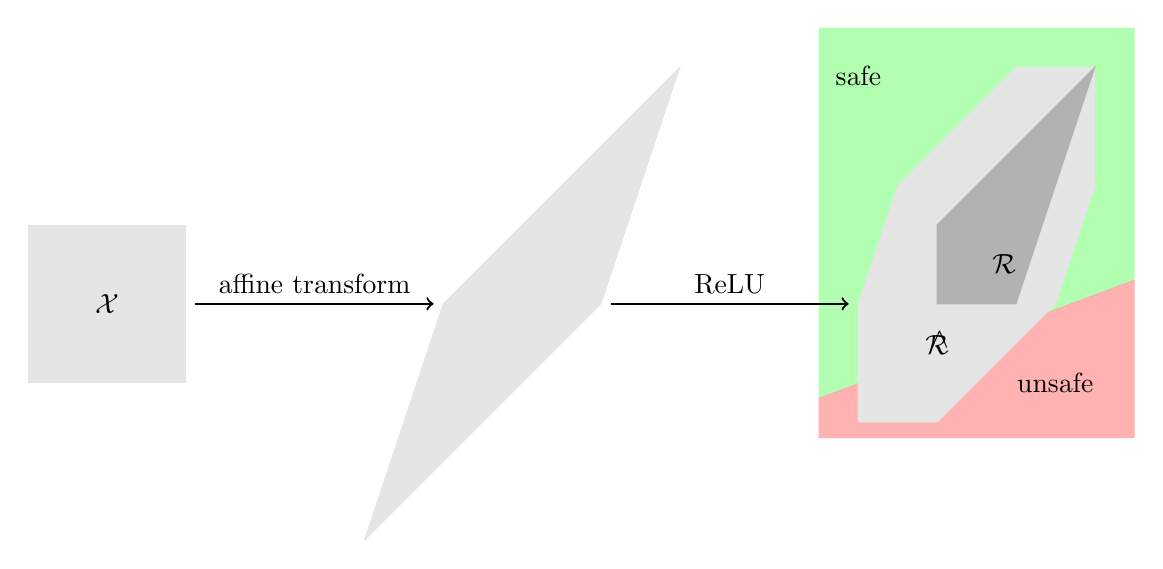
\begin{tikzpicture}[yscale=1]

	\newcommand\SSquare{+(-1.5,-2) rectangle +(2.5,3.5)}

\begin{scope}
	\draw[fill=black!10!white, color=black!10!white]  (-1,-1) --
(-1,1) -- (1,1) -- (1,-1) -- (-1,-1);	
\node at (0,0) {$\mathcal X$};
\node at (1,0) (p) {};
\end{scope}

\begin{scope}[xshift=15em]
	\draw[fill=black!10!white, color=black!10!white] (-2,-3) --
	(1,0) -- (2,3) -- (-1,0) -- (-2,-3);	
	\node at (-1,0) (p2) {};
	\node at (1,0) (p3) {};
\end{scope}

\begin{scope}[xshift=30em]
	%\draw[fill=black!10!white, color=black!10!white] (0.5,1.5) --
	%(2,3) -- (1.5,1.5) -- (0,0);
	%\draw[fill=black!10!white, color=black!10!white] (-0.5,0) --
	%(1,1.5) -- (0.5,0) -- (-1,-1.5);
	%\draw[fill=black!10!white, color=black!10!white] (0.5,0) --
	%(2,1.5) -- (1.5,0) -- (0,-1.5);
	%\draw[fill=black!10!white, color=black!10!white] (-0.5,1.5) --
	%(1,3) -- (0.5,1.5) -- (-1,0);

	\draw[color=green!30!white,fill=green,fill opacity=0.3] (-1.5,-1.2) --
	(2.5,0.3) -- (2.5,3.5) -- (-1.5,3.5) -- (-1.5,-1.2);

	\draw[color=red!30!white,fill=red,fill opacity=0.3] (-1.5,-1.2) --
	(2.5,0.3) -- (2.5,-1.7) -- (-1.5,-1.7) -- (-1.5,-1.2);

	%\draw[color=green,fill=green,fill opacity=0.1]  \SSquare;

	\draw[fill=black!10!white, color=black!10!white] (-0.5,1.5) --
	(1,3) -- (2,3) -- (2,1.5) -- (1.5,0) -- (0,-1.5) -- (-1,-1.5) --
	(-1,0) -- (-0.5,1.5);

	\draw[fill=black!30!white, color=black!30!white] (0,1) -- (2,3) --
	(1,0) -- (0,0) --  (0,1);

	%\draw[pattern=dots, pattern color=black]  (-0.5,1.5) --
	%(1,3) -- (2,3) --  (2,2)  -- (-1,-1) -- (-1,0) -- (-0.5,1.5);
	
	\node at (0,-0.5) {$\mathcal{\hat R}$};
	\node at (0.85,0.5) {$\mathcal{ R}$};
	\node at (1.5,-1) {unsafe};
	\node at (-1,2.9) {safe};

	\node at (-1,0) (p4) {};


\end{scope}

\draw[->,thick] (p) -- node[above] {affine transform} (p2);
\draw[->,thick] (p3) -- node[above] {ReLU} (p4);

	%\draw[->] (3.75,0) -- node[above,font=\scriptsize] {weighted sum}
	%(5.75,0);
	%\draw[fill=black!10!white, color=black!10!white] (6,-1) --
	%(8.5,-1) -- (8.5,1) -- (6,1) -- (6,-1);
	%\draw[fill=black!30!white, color=black!30!white] (6,-1) -- (8,0)
	%-- (8.5,1) -- (6.5,0) -- (6,-1);


	%\draw[->] (8.75,0) -- node[above,font=\scriptsize] {ReLU}
	%(9.75,0);
	%\draw[fill=black!10!white, color=black!10!white] (10,0) -- (12.5,0)
	%-- (12.5,1) -- (10,1) -- (10,0);
	%\draw[fill=black!30!white, color=black!30!white] (10,0) -- (12,0) --
	%(12.5,1) -- (10.5,0) -- (10,0);




  %\newcommand\Square{+(-1,-1) rectangle +(1,1)}

  %% Draw first rectangle and name
  %\node at (4,0.5) {$I_1$};
  %\node[label=$p$]  (p) at (3,4) {};
  %% Fill square
  %\draw[fill=blue,fill opacity=0.1] (p) \Square;
  %%\draw[->,>=latex] (p) ++(-1,-1) -- ++(2.5,0);
  %%\draw[->,>=latex] (p) ++(-1,-1) -- ++(0,2.5);
  %\fill[orange] (p) circle (2.5pt);

  %% Draw next rectangle
  %\begin{scope}[xshift=10cm]

    %\draw (0,0) rectangle (8,6);
    %\node at (4,0.5) {$I_2$};
    %\node[label=$p'$] (p') at (3,4) {};
    %\fill[orange] (p') circle (2.5pt);

	%\node at (-1,-1) {$x$};
	%\begin{scope}[cm={1.5,0.5,1.5,1.5,(0,0)}]
      %\draw[fill=blue,fill opacity=0.1] (p') \Square;

    %\end{scope}

  %\end{scope}

  %\draw[thick,->] (p) edge[bend right] (p');



	%\draw[fill=black!10!white, color=black!10!white] (2.5,-0.5) --
	%(3.5,-0.5) -- (3.5,0.5) -- (2.5,0.5) -- (2.5,-0.5);	
	
	%\draw[->] (3.75,0) -- node[above,font=\scriptsize] {weighted sum}
	%(5.75,0);
	%\draw[fill=black!10!white, color=black!10!white] (6,-1) --
	%(8.5,-1) -- (8.5,1) -- (6,1) -- (6,-1);
	%\draw[fill=black!30!white, color=black!30!white] (6,-1) -- (8,0)
	%-- (8.5,1) -- (6.5,0) -- (6,-1);


	%\draw[->] (8.75,0) -- node[above,font=\scriptsize] {ReLU}
	%(9.75,0);
	%\draw[fill=black!10!white, color=black!10!white] (10,0) -- (12.5,0)
	%-- (12.5,1) -- (10,1) -- (10,0);
	%\draw[fill=black!30!white, color=black!30!white] (10,0) -- (12,0) --
	%(12.5,1) -- (10.5,0) -- (10,0);

	%\draw[pattern=north west lines, pattern color=black] (10,0)  --
	%(12.5,1) -- (12.5,0) -- (10,0);

	%\node[xshift=8.5em] {$\mathcal X$};
	%\node[xshift=29.5em,yshift=2em] {$\mathcal{\hat R}$};
	%\node[xshift=33em,yshift=0.5em] {$\mathcal{ R}$};
	%\node[xshift=35em,yshift=0.5em] {$\mathcal{ Y}$};



\end{tikzpicture}
}

